\begin{center}
  
  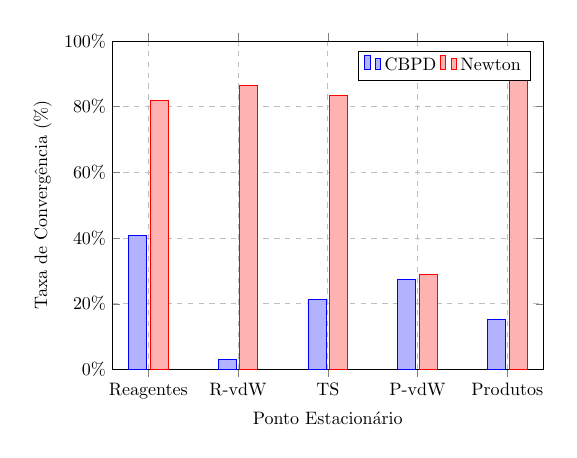
\begin{tikzpicture}[scale = 0.65]
    \begin{axis}[
      width=10cm,
      height=8cm,
      xlabel={Ponto Estacionário},
      ylabel={Taxa de Convergência (\%)},
      xtick=data,
      xticklabels={Reagentes, R-vdW, TS, P-vdW, Produtos},
      legend style={at={(0.5,-0.2)}, anchor=north, legend columns=-1},
      ymin=0,
      ymax=100,
      grid=major,
      grid style=dashed,
      ymajorgrids=true,
      ybar,
      ytick={0,20,...,100},
      yticklabel={\pgfmathprintnumber{\tick}\%},
      legend pos=north east
    ]

      \addplot[color=blue, fill=blue!30] coordinates {
        (1, 40.91)
        (2, 3.03)
        (3, 21.21)
        (4, 27.27)
        (5, 15.15)
      };

      \addplot[color=red, fill=red!30] coordinates {
        (1, 81.82)
        (2, 86.36)
        (3, 83.33)
        (4, 28.79)
        (5, 93.94)
      };

      \legend{CBPD, Newton}

    \end{axis}
  \end{tikzpicture}

\end{center}
